\documentclass[10pt,a4paper]{article}
\usepackage[utf8x]{inputenc}
\usepackage{ucs}
\usepackage{amsmath}
\usepackage{amsfonts}
\usepackage{amssymb}
\usepackage{eurosym}
\usepackage[english]{varioref}
\usepackage{setspace}
\usepackage{listings}
\usepackage[
    pdftex,
    a4paper,
    bookmarks,
    bookmarksopen=true,
    pdfauthor={Daniel Otte},
    pdftitle={AnonAccess},
  %  colorlinks,
  %  linkcolor=blue,
  %  urlcolor=blue,
    bookmarksnumbered=true,hyperindex=true]{hyperref}
%% for producing ps use dvips for pdfs use pdftex
%\usepackage[dvips]{graphicx} 
\usepackage[pdftex,final]{graphicx}
\usepackage{picins}
\usepackage{picinpar}
\usepackage{algorithmic}
\usepackage{algorithm}

\author{Daniel Otte\\daniel.otte@ruhr-uni-bochum.de \and Sören Heisrath\\sh@3dots.de }
\title{\Huge{\textsf{AnonAccess}} \\ \normalsize{das Labor \\ \url{http://www.das-labor.org}}}

%-----

\begin{document} 

\begin{figure}[t]
 \begin{minipage}[b]{.3\linewidth}
 
\includegraphics[scale=0.15]{Labor} 
 \end{minipage}
 \hspace{0.3\linewidth}
 \begin{minipage}[b]{.3\linewidth}
 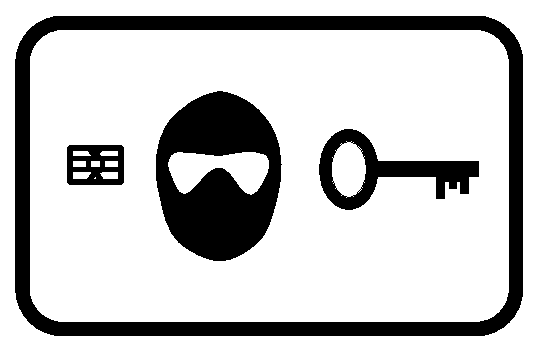
\includegraphics[scale=0.7]{AnonAccessLogo} 
 \end{minipage}
\end{figure}

\maketitle

\begin{abstract}
This paper gives an overview of the AnonAccess-system, which tries to provide access to users which may be known by name, pseudonym or a shared pseudonym, to a given functionality (ex. open a door). The shared pseudonym access feature is tried to be extended and implemented in such a way that it can be claimed to be anonymous.
\end{abstract}

\section{Notations and conventions}
\begin{tabular}{ll}
$a \oplus b$ & $a$ xor $b$ \\
$a \wedge b$ & $a$ bit wise and $b$ \\
$a \vee b$ & $a$ bit wise or $b$ \\
$a \parallel b$ & concatenation of the bit strings $a$ and $b$ \\
$a_{(base)}$ & the constant $a$ is given in base $base$ notation, if not specified the base is 10\\
$H(a)$ & is the value of the hash function SHA-256 of message $a$ \\
$HMAC_{key}(a)$ & is the value of the HMAC-SHA256 MAC function of message $a$ and key $key$ \\
$bit$ & a bit is the basic unit of information; it can only have one of two values, \\ 
& which we consider to be 1 and 0 \\
$byte$ & a byte is considered to be a group of eight bits throughout this document \\
Ki, Mi, Gi & prefixes to units, specifying a multiple of $2^{10} = 1,024$, $2^{20} = 1048,576$ and\\ & $2^{30} = 1,073,741,824$; see \cite{IEC60027-2} for reasons \\
K, M, G & prefixes to units, specifying a multiple of $10^3 = 1,000$, $10^6 = 1,000,000$ and\\ & $10^9=1,000,000,000$ \\ 
\end{tabular}
\section{Cryptographic algorithms used}
We use the following cryptographic primitives:
\begin{itemize}
 \item SHA-256 hash function as specified in \cite{FIPS180-2}
 \item HMAC-SHA256 MAC function as specified in \cite{RFC2104}
 \item Shabea with 16 rounds as data encryption algorithm as specified in appendix B
 \item a PRNG as specified in appendix A
\end{itemize}
\section{Components}

\subsection{Chip-Card}
We use simple memory cards with $I^2$C-Bus and form factor ID-00 as specifyed in ISO 7816. They are quite cheap (less then 1\euro{} per Card) and are not secure. Their contents might be easily read or modifyed. So everyone can read and check what we write on their card.

%-----

\subsection{realtimeclock (RTC)}
The realtimeclock is implemented in software by using one of the microcontrollers timers. A timerinterrupt function increments a 64bit value every millisecond (this counter will wrap arround in about 584.542.046 years, which should be quite enough for us). Additionaly the counters value is periodically\footnote{the value is backed up every $3FFFFF_{(16)}$ milliseconds wich is about every 1.165 hours} written to the microcontrollers eeprom and read back after reset. On reset we also add the value $3FFFFF_{(16)}$ to the counter to avoid having more then on time the same timestamp.

\subsection{random number generator (RNG)}
\begin{window}[0,r, 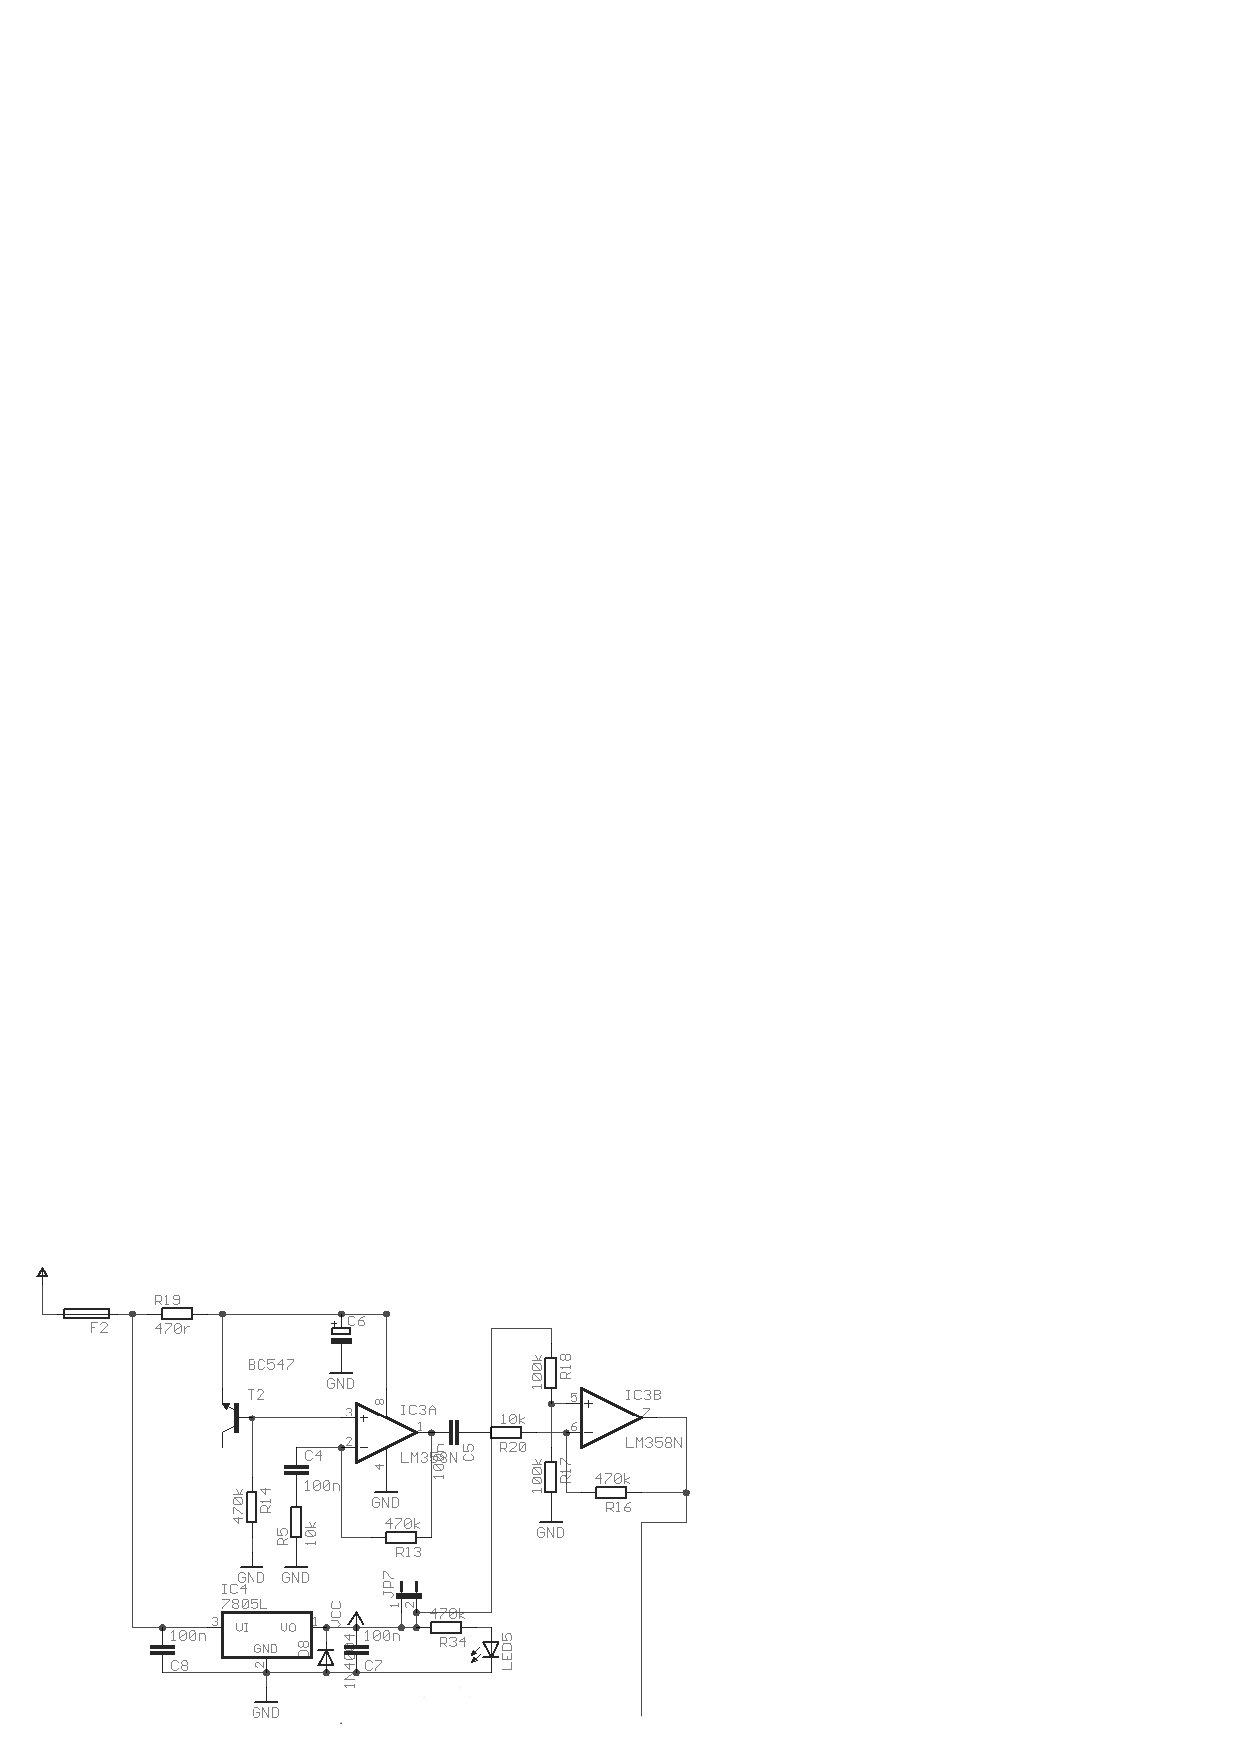
\includegraphics[scale=0.5]{RNG}, {schematic of the hardware random generator}]
This curcit utilises the randomnes of the breakthrough voltage of the diode of a transistor to generate random voltages in the range from 0 to 5 volts. While this is quite random it does not need to be cryptographicaly secure because the RNGs output is used only as input for the cryptograpicaly secure PRNG. \\
\{bla, bla, bla, bla, bla, bla, bla, bla, bla, bla, bla, bla, bla, bla, bla, bla, bla, bla, bla, bla, \}
\end{window}
%-----

\subsection{pseudornadom number generator (PRNG)}
The PRNG is based on the SHA-256 hash function and is specified in Appendix A.
It has two main functions:
\begin{itemize}
 \item AddEntropy: this function adds data to the entropy pool, the input can be of arbitary bit length
 \item GetRandomBlock: this function fills a 32 byte block of memory with a randomised bitstring
\end{itemize}
An other function (GetRandomByte) uses a buffer and the GetRandomBlock function and returns a random byte.
The PRNG is periodicaly filled with entropy from the hardware RNG using the AddEntropy function.
%-----

\subsection{secure serial port (QPort-tiny)}

%-----

\subsection{external serial eeprom}
The external serial eeprom is used to keep the two databases and can be used for key-exporting for migration. We use standard $I^2C$ EEPROMs with 512Kbit or 1Mbit (24xx512 or 24xx1025) from Microchip. It is possible to extend the storage capabilitys by using multiple EEPROMs. This makes it possible to have up to 4Mbit or 512Kbytes of storage space wich normally allows more than 10.000 users.

The whole contents of the eeprom is encrypted (except the keymigration-area). Shabea-16 is used to encrypt the content. We therfore divide the eeprom space into 32 byte blocks which are encrypted seperatly. Every block is encrypted with an individual key which is the result of concatenation of the ''main-key'' and the blockaddress. So we are protected against most attacs against massstorage-encryption (ex. watermarking) 

%-----

\subsection{Ticket-Database (TicketDB)}
This database is used to store a HMAC of the users ticket, her/his permissions, and some statistics about the whole system.
The first element in the database is the header followe by the entrys for the users.\\
\begin{tabular}{|l|c|l|}\hline 
name & size & description \\ \hline
ID & 10 bytes & set to the string ''AnonAccess'' \\
majversion & 1 byte & majorversion; set to 1 \\
minversion & 1 byte & minorversion; set to 0 \\
headersize & 1 byte & specifies the size of the header \\
stat & 10 bytes & statistics \\
reserved & 8 bytes & reserved field for future extensions and for alignement; set to 0 \\ \hline
\end{tabular} 


 the statistics field has the following structure:\\
\begin{tabular}{|l|c|l|} \hline
name & size & description \\ \hline 
max\_users     & 2 bytes & maximum number of users \\
users              & 2 bytes & actualy active user \\
admins           & 2 bytes & actualy active admins \\
locked\_users   & 2 bytes & number of locked users \\
locked\_admins & 2 bytes & number of locked admins \\ \hline
\end{tabular} 

The following space of the ticketDB is filled with userentrys which have the following structure:\\
\begin{tabular}{|l|c|l|} \hline
name & size & description \\ \hline 
flags         & 1 byte    & the flags associated with the user \\
nickname  & 7 bytess & the nickname if the user decided to be known by name \\
ticketmac  & 32 bytes & HMAC from users ticket \\ \hline
\end{tabular} 

Where the flag field has the following structure: \\
\begin{tabular}{|l|c|l|} \hline
name & size & description \\ \hline 
exists         & 1 bit    &  indicates if this entry is used (1: in use; 0: free)\\
admin  & 1 bit & set if user has admin privileges, cleared othewise \\
locked  & 1 bit & set if user is locke; cleared otherwise \\
noitfy\_lostadmin  & 1 bit & set if user has to be notifyed about lost admin privileges \\
anonymous  & 1 bit & set if the user did not specify username to be stored \\
reserved & 3 bit & reserved, should be set to 0\\ \hline
\end{tabular} 


%-----

\subsection{FlackModifying-Database (FLMDB)}





\section{Being known by name or shared pseudonym}
AnonAccess allows three ways of being known:
\begin{itemize}
\item being known by name
\item being known by pseudonym
\item being known by a shared pseudonym
\end{itemize}

\subsection{Being known by name}
If the user selects to be known by name the nickname is stored in the \textit{TicketDB} in a way that is available in plaintext to the \textit{Master-Unit}. It can be searched for and it can be read by an administrator. This allows immediate manipulation of the user's flags.

\subsection{Being known by pseudonym}
In every mode the user enters his/her nickname at card creation time at the \textit{Terminal-Unit}, and the \textit{Master-Unit} generates a HMAC (with a special key, the \textit{nickkey}) from this nickname. This HMAC is referred to as \textit{user pseudonym} in this document. It is neither possible for the \textit{Master-Unit} nor the \textit{Terminal-Unit} to compute the user's nickname from this pseudonym. The \textit{user pseudonym} is not stored in the \textit{Master-Unit} neither in the \textit{Terminal-Unit}, it is stored only in double encrypted form in the \textit{AuthBlock} on the users card.

This pseudonym is used to apply modifications to a given account. A modification is done by adding an entry to the \textit{FLMDB}. As this requires the \textit{user pseudonym}, the nickname of the associated user must be known. Also the modifications can only be applied when the user processes the user authentication process.

\subsection{Sharing a pseudonym}
It is also possible to have multiple users sharing the same \textit{user pseudonym}. Therefore they simply have to enter the same nickname. It is recommended to use the name of colors for such groups.

To apply modifications to an account in such a group, the modification has to be applied to all members of the group. An exception is the case where the card related to this account is available. In this case the \textit{UID} from the card can be used to modify the flags in the \textit{TicketDB} directly.

\section{Usage}
This section describes the AnonAccess system from the user point of view.

%-----

\subsection{Admin status}

%-----

\subsection{Actions and commands}

\section{Ideal run}
 \begin{enumerate}
 \item User inserts card in \textit{Terminal-Unit}
 \item \textit{Terminal-Unit} reads \textit{AuthBlock} from card and transmits it in \textit{addAuth}-Packet to \textit{\textit{Master-Unit}}
 \item \textit{Master-Unit} checks \textit{UID} to be in range
 \item \textit{Master-Unit} checks \textit{ticket} against the HMAC in \textit{TicketDB} at \textit{UID}
 \item \textit{Master-Unit} loads \textit{userflags} from \textit{TicketDB}
 \item \textit{Master-Unit} decrypts \textit{ticket} and checks \textit{timestamp} to be in range
 \item \textit{Master-Unit} decrypts \textit{$r_{ID}$} ($dec_{pseudokey}(dec_{r_{key}}(r_{ID}))$) to get users pseudonym
 \item \textit{Master-Unit} searches in \textit{FLMDB} for entries matching users pseudonym; for every matching entry it does:
  \begin{enumerate}
  \item modify users flags as indicated by the \textit{setflags} and \textit{clearflags} fields
  \item delete the entry if the \textit{permanent}-flag is not set
  \end{enumerate}
 \item \textit{Master-Unit} deletes \textit{TicketDB}-entry
 \item \textit{Master-Unit} generates a new \textit{UID} which points to an entry in \textit{TicketDB}
 \item \textit{Master-Unit} generates a new \textit{ticket} with a new \textit{timestamp}
 \item \textit{Master-Unit} writes new \textit{ticket} at \textit{UID} in \textit{TicketDB}
 \item \textit{Master-Unit} generates new \textit{$r_{key}$}
 \item \textit{Master-Unit} generates new \textit{$r_{ID}$}$=enc_{rid\_key}(enc_{r_{key}}(users pseudonym))$ 
 \item \textit{Master-Unit} transmits new \textit{AuthBlock} in \textit{addAuthAck}-Packet to \textit{Terminal-Unit}
 \item \textit{Terminal-Unit} writes new \textit{AuthBlock} onto card
 \end{enumerate}

\section{Attacks and trusted components}
This section tries to give an overview of the trust level of components and thereby an overview of the trust level of a complete implementation of AnonAccess.

\subsection{Security goals}
\begin{itemize}
 \item access should only be granted to users who have a valid card whichs information and related information in the database state, that access should be granted to this user.
 \item no valuable information should be retrievable from the card's contents
 \item no valuable information should be retrievable by an unauthorised user from the AnonAccess system
 \item no information about the presence of a user who is not known by nickname should be available, even to an user with admin privileges
\end{itemize}

\subsection{Trusted components}
We consider a component to be a trusted component if the compromisation of this component leads to compromisation of at least one of the former declared security goals.

\subsubsection{Terminal-Unit}
The \textit{Terminal-Unit} is considered trusted, especially the connection between the microcontroller and the card must be protected.

\subsubsection{Master-Unit}
The \textit{Master-Unit} is considered trusted, especially the serial bus between the microcontroller and the external serial EEPROM must be protected. Although the external EEPROM's content is encrypted, an attacker might gather usefull information from the addresses which are accessed.

 

\begin{appendix}
\section{the PRNG}
our PRNG utilises the SHA-256 function
\begin{figure}
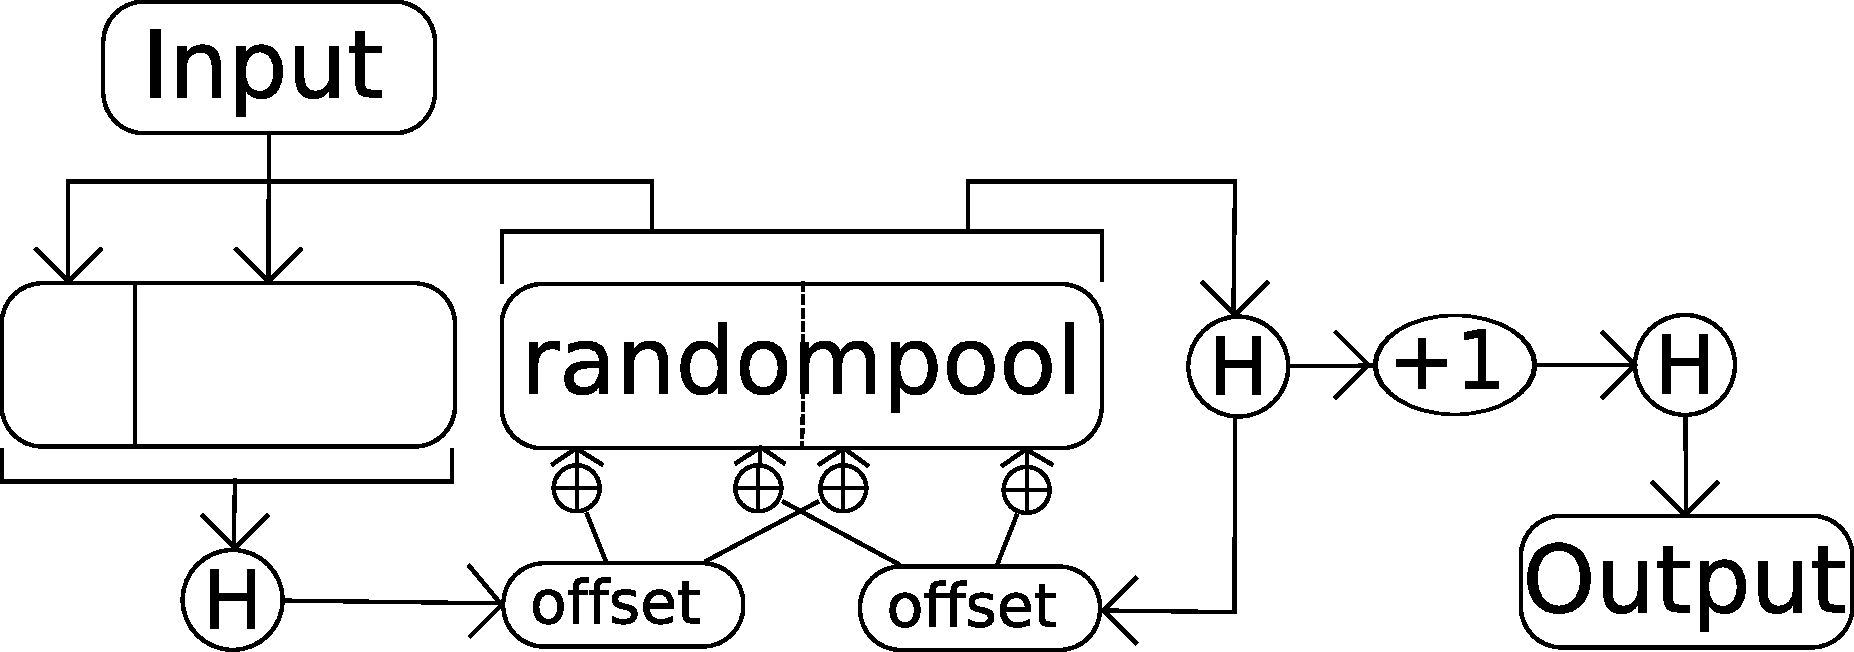
\includegraphics[scale=0.3]{PRNG} 
\caption{schematic of the PRNG}
\end{figure}
\section{the Shabea-Cipher}
Shabea (SHA based encryption algorithm) is a SHA-256 based Feistel-Cipher. It was designed to securely encrypt data where a SHA-256 implementation is available. It was important to have a small (in program space and memory requirement) and nevertheless secure symmetric cipher, in the case that a SHA-256 implementation is available.

\begin{algorithm}
\caption{Encryption with Shabea}
\label{algShabeaEnc}
\begin{algorithmic}
\REQUIRE $INPUT = L_0 \parallel R_0$ where $L_0$ and $R_0$ are both 16 bytes large
\REQUIRE $4\leq rounds\leq 255$
\REQUIRE $key$ which length (in bits) is $keylength$ of any size
\FOR{$i=0$ to $rounds$}
\STATE $L_{i+1} \leftarrow R_i$
\STATE $R_{i+1} \leftarrow L_i \oplus H(key \parallel 0 \parallel i \parallel R_i)$
\ENDFOR
\STATE $OUTPUT = L_{i+1} \parallel R_{i+1}$
\end{algorithmic}
\end{algorithm}

\begin{algorithm}
\caption{Decryption with Shabea}
\label{algShabeaDec}
\begin{algorithmic}
\REQUIRE $INPUT = L_{rounds} \parallel R_{rounds}$ where $L_{rounds}$ and $R_{rounds}$ are both 16 bytes large
\REQUIRE $4\leq rounds\leq 255$
\REQUIRE $key$ which length (in bits) is $keylength$ of any size
\FOR{$i=rounds+1$ downto $1$}
\STATE $R_{i-1} \leftarrow L_i$
\STATE $L_{i-1} \leftarrow R_i \oplus H(key \parallel 0 \parallel i \parallel L_i)$
\ENDFOR
\STATE $OUTPUT = L_0 \parallel R_0$
\end{algorithmic}
\end{algorithm}

\end{appendix}
 
\newpage

\begin{thebibliography}{999}
 \bibitem{IEC60027-2}When is a kilobyte a kibibyte? And an MB an MiB? (\url{http://www.iec.ch/zone/si/si_bytes.htm})

 \bibitem{FIPS180-2}FIPS 180-2: Secure Hash Standard (SHS) (\url{http://csrc.nist.gov/publications/fips/fips180-2/fips180-2withchangenotice.pdf})
 
 \bibitem{RFC2104}RFC 2104: HMAC: Keyed-Hashing for Message Authentication

 \bibitem{I2C}The $I^2C$-Bus Specification, Version 2.1, January 2000, original specification from NXP Semiconductors (\url{http://www.nxp.com/acrobat_download/literature/9398/39340011.pdf})
 
 \bibitem{ISO7816-1}ISO/IEC 7816-1:1998 Identification cards -- Integrated circuit(s) cards with contacts -- Part 1: Physical characteristics

 \bibitem{ISO7816-2}ISO/IEC 7816-2:1999 Identification cards -- Integrated circuit cards -- Part 2: Cards with contacts -- Dimensions and location of the contacts

 \bibitem{ASN.1BER}ITU-T Rec. X.690: Information technology ? Abstract Syntax Notation One (ASN.1): Specification of basic notation (\url{http://www.itu.int/ITU-T/studygroups/com17/languages/X.680-0207.pdf})

 \bibitem{24xx512} 24AA512/24LC512/24FC512 1024K $I^2C$ CMOS Serial EEPROM, datasheet by Microchip (\url{http://ww1.microchip.com/downloads/en/DeviceDoc/21754H.pdf})

 \bibitem{24xx1025} 24AA1025/24LC1025/24FC1025 1024K $I^2C$ CMOS Serial EEPROM, datasheet by Microchip (\url{http://ww1.microchip.com/downloads/en/DeviceDoc/21941E.pdf})

 \bibitem{microchip}The Microchip Cooperation web presence (\url{http://www.microchip.com})

 \bibitem{QPort-tiny}QPort-tiny specification, not written yet.

 \bibitem{XTEA}Tea extensions, Roger M. Needham and David J. Wheeler, (Notes October 1996, Revised March 1997,      Corrected October 1997) (\url{http://www.cix.co.uk/~klockstone/xtea.pdf})

 \bibitem{Atmel}The Atmel Cooperation web presence (\url{http://www.atmel.com})  

 \bibitem{ATmega644}ATmega644 Preliminary (revision M, updated 08/07)  (\url{http://www.atmel.com/dyn/resources/prod_documents/doc2593.pdf})

 \bibitem{ATmega32}ATmega32(L) (revision K, updated 08/07)  (\url{http://www.atmel.com/dyn/resources/prod_documents/doc2503.pdf})

 \bibitem{GCC}GCC, the GNU Compiler Collection (\url{http://gcc.gnu.org})
 
 \bibitem{AVR-Libc}AVR Libc Home Page (\url{http://www.nongnu.org/avr-libc/})
\end{thebibliography}

\end{document}